%%%%%%%%%%%%%%%%%%%%%%%%%%%%%%%%%%%%
% Header                           %
%%%%%%%%%%%%%%%%%%%%%%%%%%%%%%%%%%%%
% 
% Revisions: 2017-04-10 Martin R�del <martin.raedel@dlr.de>
%                       Initial draft
%               
% Contact:   Martin R�del,  martin.raedel@dlr.de
%            DLR Composite Structures and Adaptive Systems
%          
%                                 __/|__
%                                /_/_/_/  
%            www.dlr.de/fa/en      |/ DLR
%
%%%%%%%%%%%%%%%%%%%%%%%%%%%%%%%%%%%%
% Content                          %
%%%%%%%%%%%%%%%%%%%%%%%%%%%%%%%%%%%%

\levelstay{Display point/node numbers}
\label{sec:Paraview:Display:Point:Labels}

After importing the model it might be of interest to get the node/point numbers for the whole model or a specific selection. To show these numbers after importing the model:

\begin{enumerate}[noitemsep]
  \item Generate and extract the selection of interest according to \autoref{sec:Use_ParaView_Selection}
  \item Left-click on the imported model (set the model active)
  \item From the menubar:
    \begin{itemize}[noitemsep]
      \item Click \textit{View}
      \item Click \textit{Selection Display Inspector}
    \end{itemize}
  \item In the \textit{Selection Display Inspector} window:
    \begin{itemize}[noitemsep]
      \item Click on \textit{Point Labels}
      \item Select \textit{ID}
    \end{itemize}
  \item The point/node numbers appear as labels
\end{enumerate}

\begin{figure}[htbp]
\centering
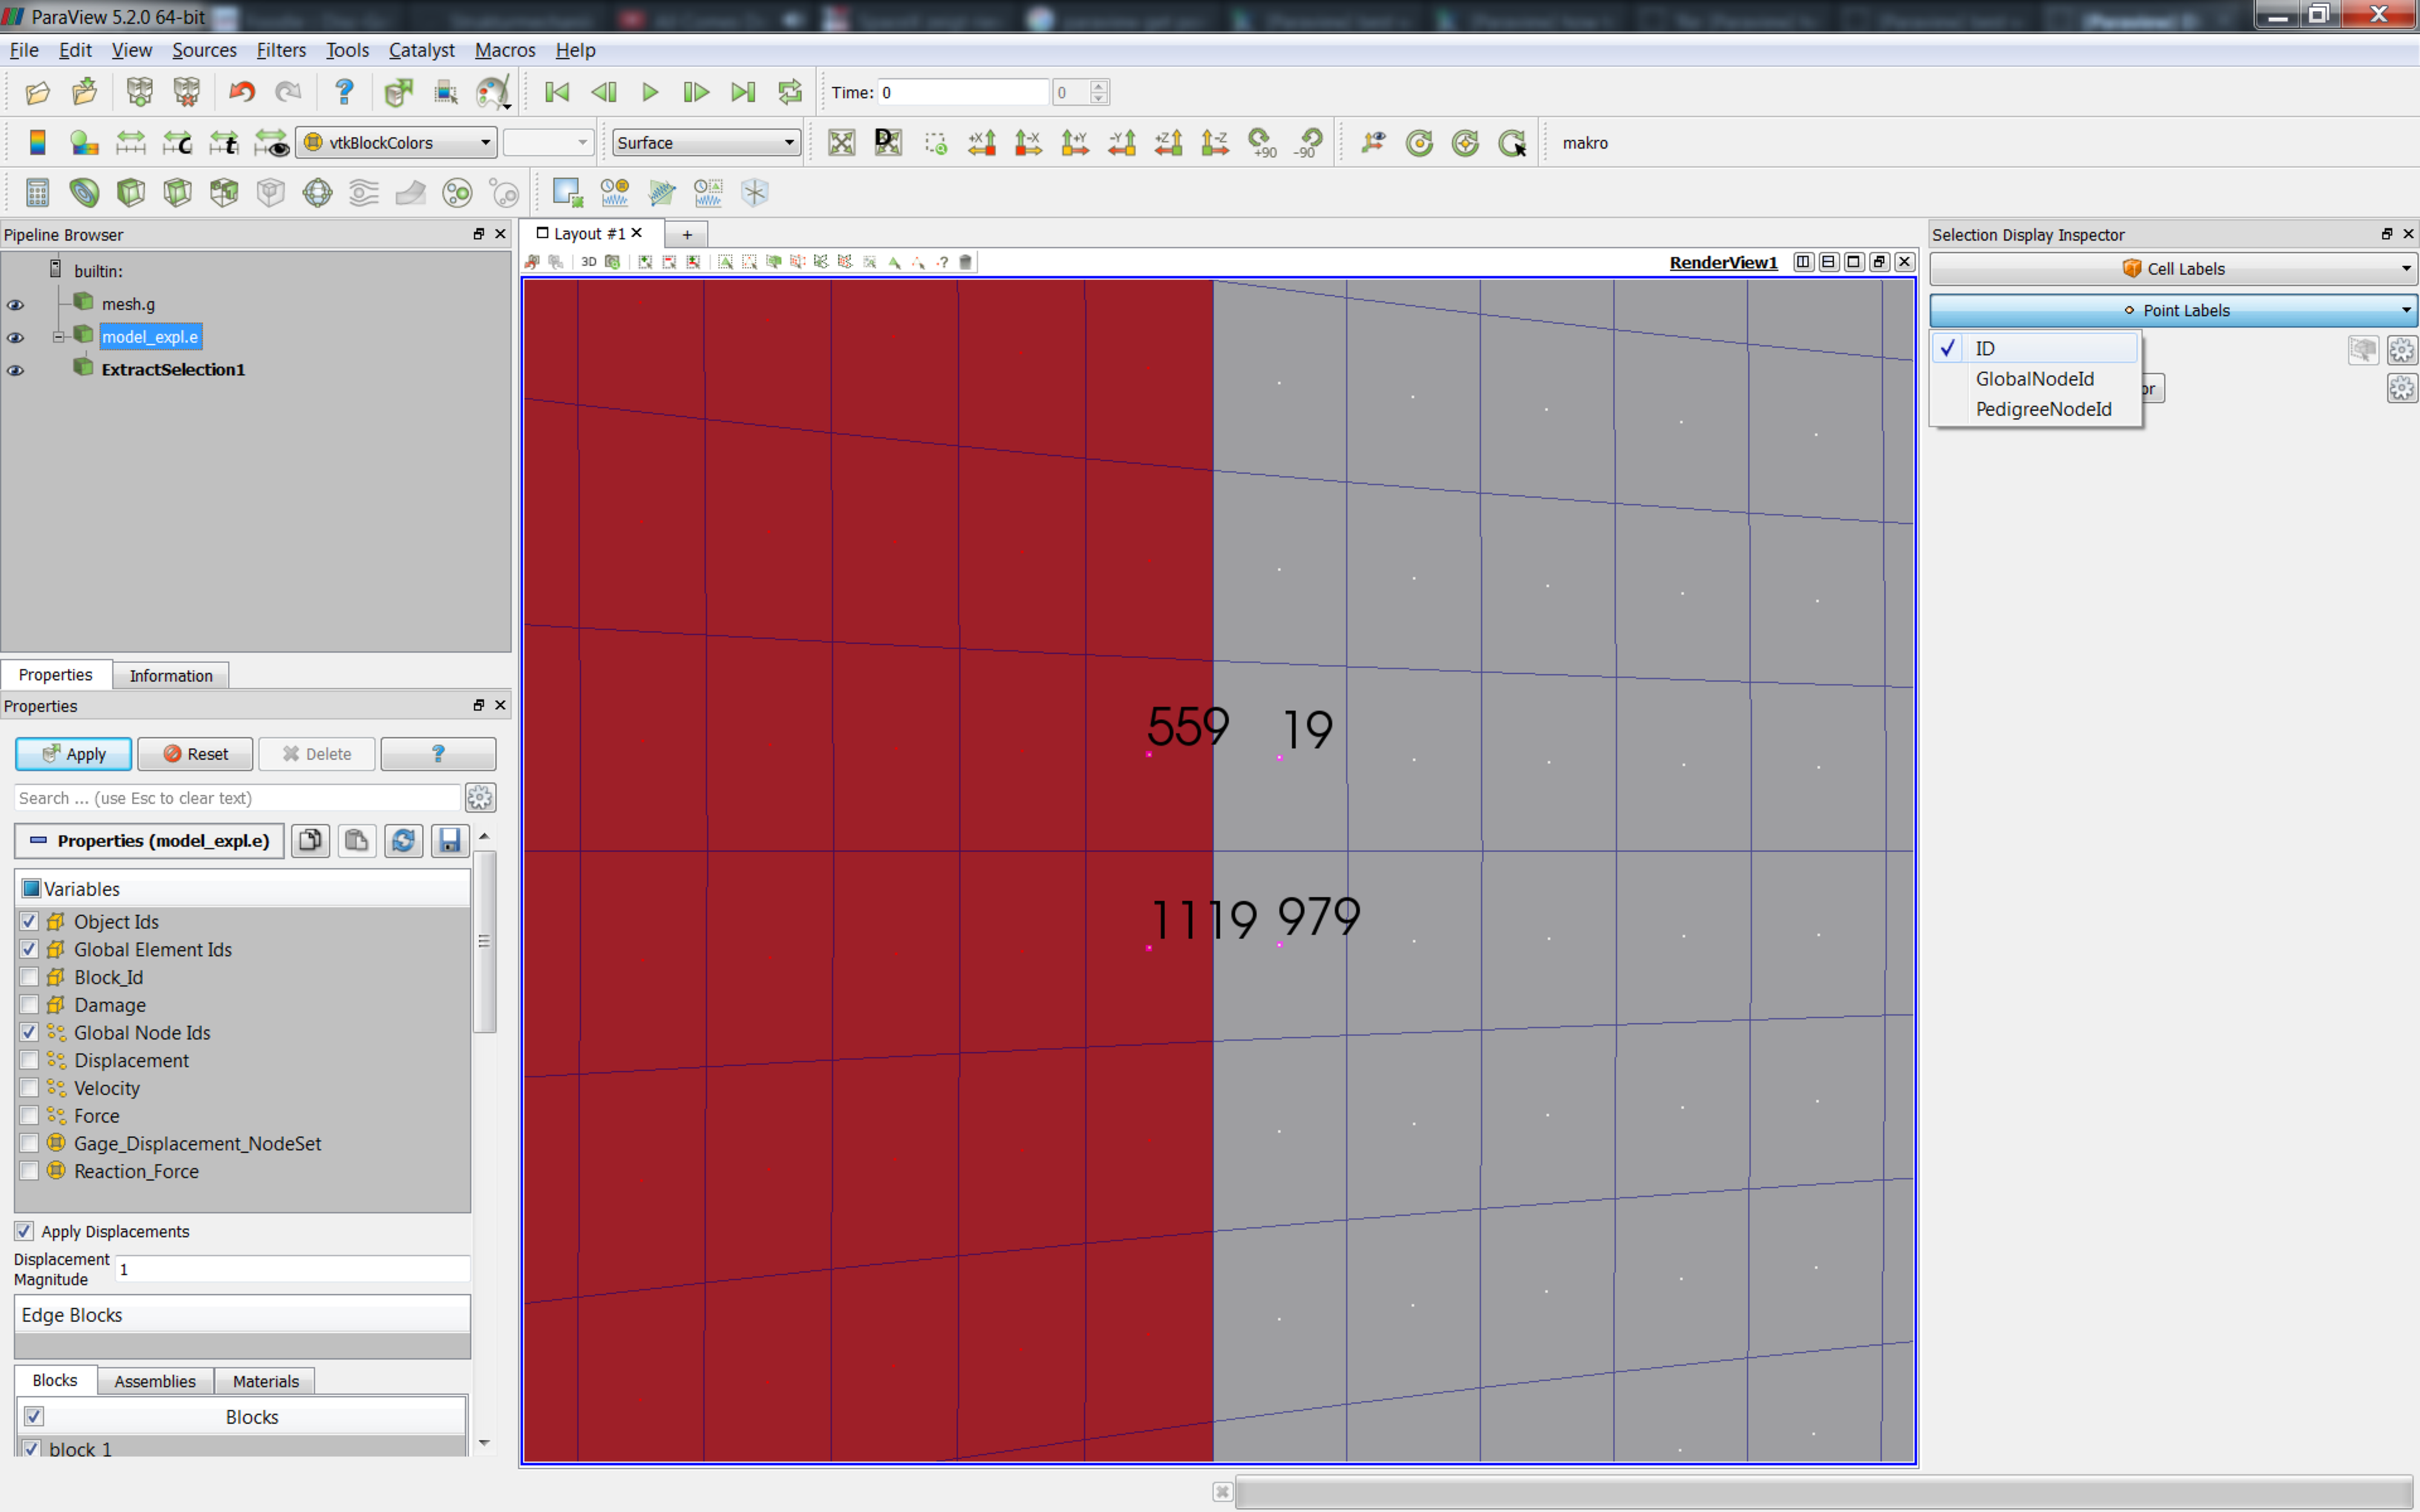
\includegraphics[width=\paraviewscreenshotwidthfac\linewidth]{Figures/Screenshots/ParaView_Display_NodeLabels}
\caption{Display of selection point/node numbers}
\label{fig:Use_ParaView_Display_NodeLabels}
\end{figure}
